\lecture{5.4}{Cross-Validated Risk Assessment}
\label{lec:5-4}

\subsection{The Problem with Empirical Risk}

The population risk
\[
R(\Qbar_n)=\E\{L(\Qbar_n)(W,A,Y)\}
\]
cannot be computed directly because the true distribution of $(W,A,Y)$ is unknown.
A tempting estimate is the empirical risk on the same data used to fit $\Qbar_n$:
\[
R_n(\Qbar_n)
=
\frac{1}{n}\sum_{i=1}^n
L(\Qbar_n)(W_i,A_i,Y_i).
\]
For squared-error loss, this is
\[
R_n(\Qbar_n)
=
\frac{1}{n}\sum_{i=1}^n
\{Y_i-\Qbar_n(A_i,W_i)\}^2.
\]

The problem is that $\Qbar_n$ was trained to fit these same observations. A flexible
method can make training errors very small without learning a relationship that
generalizes to new data.

\subsection{Overfitting}

Overfitting occurs when an estimator captures idiosyncratic noise in the training data
instead of the stable signal in the population. A twentieth-degree polynomial may
thread through the observed data points and have very low training error, while a
third-degree polynomial may better approximate the true regression function on new
observations.

Training error is therefore often optimistic. It can also select the wrong method:
the method with the lowest empirical risk on the training data may have worse risk in
the population.

\begin{keyidea}
To evaluate prediction performance fairly, predictions should be tested on
observations that were not used to fit the prediction rule.
\end{keyidea}

\subsection{Training and Validation Samples}

Cross-validation mimics external validation by splitting the observed sample into two
roles:
\begin{itemize}
\item a training sample used to fit the regression estimator;
\item a validation sample used only to evaluate prediction loss.
\end{itemize}

If $\Qbar_{n,T}$ is fit using training set $T$ and evaluated on validation set $V$, the
validation risk estimate is
\[
R_{n,V}(\Qbar_{n,T})
=
\frac{1}{|V|}\sum_{i\in V}
L(\Qbar_{n,T})(W_i,A_i,Y_i).
\]
Because the validation observations were not used to fit $\Qbar_{n,T}$, this estimate
is a more honest measure of out-of-sample predictive performance.

\subsection{V-Fold Cross-Validation}

In $V$-fold cross-validation, the data are partitioned into $V$ approximately equal
folds. Let $\mathcal V_v$ denote the validation indices in fold $v$, and let
$\mathcal T_v$ be the remaining training indices. For each fold:
\begin{enumerate}
\item fit the candidate estimator on $\mathcal T_v$;
\item predict outcomes for observations in $\mathcal V_v$;
\item compute the average validation loss in $\mathcal V_v$.
\end{enumerate}

The cross-validated risk is the average validation loss over folds:
\[
R_{CV,n}(\Qbar_n)
=
\frac{1}{V}\sum_{v=1}^V
\left[
\frac{1}{|\mathcal V_v|}
\sum_{i\in\mathcal V_v}
L(\Qbar_{n,v})(W_i,A_i,Y_i)
\right],
\]
where $\Qbar_{n,v}$ is the estimator fit without the validation fold $\mathcal V_v$.
When folds are equal size, this is equivalent to the average loss across all
out-of-fold predictions.

\begin{figure}[H]
\centering
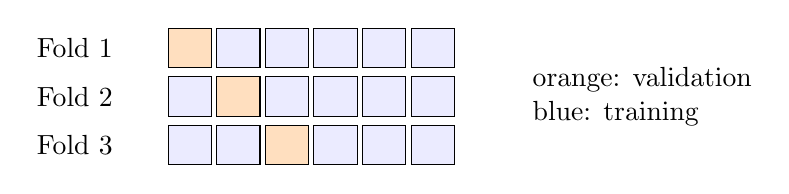
\begin{tikzpicture}[
  scale=.95,
  fold/.style={draw, minimum width=.55cm, minimum height=.5cm},
  val/.style={draw, fill=orange!25, minimum width=.55cm, minimum height=.5cm},
  train/.style={draw, fill=blue!8, minimum width=.55cm, minimum height=.5cm}
]
\foreach \r in {1,2,3} {
  \node[left] at (-.25,-.65*\r) {Fold \r};
  \foreach \c in {1,...,6} {
    \ifnum\c=\r
      \node[val] at (.65*\c,-.65*\r) {};
    \else
      \node[train] at (.65*\c,-.65*\r) {};
    \fi
  }
}
\node[align=left] at (6.7,-1.3) {orange: validation\\blue: training};
\end{tikzpicture}
\caption{In V-fold cross-validation, each fold is used once for validation.}
\label{fig:ch5-vfold}
\end{figure}

\subsection{Choosing the Number of Folds}

The number of folds controls a practical tradeoff.

With a larger $V$, each training set is closer in size to the full dataset. This can be
helpful in small samples or with flexible algorithms that need many observations to
train well. Leave-one-out cross-validation is the extreme case $V=n$.

With a smaller $V$, each validation fold is larger. This can make validation risk
estimates more stable, especially when outcomes are rare or highly skewed. Smaller
$V$ is also computationally cheaper because fewer models are fit.

Common choices include $V=5$ and $V=10$. The choice should be made before looking at
which algorithms win.

\subsection{Cross-Validated Risk as External-Data Mimicry}

The ideal way to evaluate a regression estimator would be to fit it in the study
sample and test it in a new independent sample from the same population. Such data
are rarely available. Cross-validation approximates this ideal by repeatedly creating
temporary training and validation samples from the observed data.

This matters for causal inference because nuisance functions are often selected before
being inserted into causal effect estimators. Cross-validated risk gives a pre-specified,
objective criterion for choosing among candidate outcome regressions or propensity
score models.

\begin{estimationbox}
V-fold cross-validation workflow:
\begin{enumerate}
\item Split the sample into $V$ folds.
\item For each candidate regression estimator and each fold, fit the estimator on the
training folds.
\item Predict on the held-out fold.
\item Compute validation loss.
\item Average validation loss over folds.
\item Prefer candidates with lower cross-validated risk.
\end{enumerate}
\end{estimationbox}
